%
% teil3.tex -- Resultate und Ausblick
%
% (c) 2022 Fabian Dünki, Hochschule Rapperswil
%
\section{Auswertung
\label{0f1:section:teil3}}
\rhead{Resultate}
Im Verlauf dieser Arbeit hat sich gezeigt, 
das einen einfachen mathematischen Algorithmus zu implementieren gar nicht so einfach ist.
So haben alle drei umgesetzten Ansätze Probleme mit grossen negativen $z$ in der Funktion $\mathstrut_0F_1(;c;z)$.
Ebenso kann festgestellt werden, dass je grösser der Wert $z$ in $\mathstrut_0F_1(;c;z)$ wird, desto mehr weichen die berechneten Resultate von den Erwarteten \cite{0f1:wolfram-0f1} ab.

\subsection{Konvergenz
\label{0f1:subsection:konvergenz}}
Es zeigt sich in Abbildung \ref{0f1:ausblick:plot:airy:konvergenz}, dass nach drei Iterationen ($k = 3$) die Funktionen genaue Resultate im Bereich von $-2$ bis $2$ liefert. Ebenso kann festgestellt werden, dass der Kettenbruch schneller konvergiert und im positiven Bereich mit der Referenzfunktion $\operatorname{Ai}(x)$ übereinstimmt. Da die Rekursionsformel eine Abwandlung des Kettenbruches ist, verhalten sich die Funktionen in diesem Fall gleich.

Erst wenn mehrerer Iterationen gerechnet werden, ist wie in Abbildung \ref{0f1:ausblick:plot:konvergenz:positiv} dargestellt, der Kettenbruch den anderen zwei Algorithmen bezüglich Konvergenz überlegen. Bei der Rekursionsformel muss beachtet werden, dass sie zwar erst nach 35 Approximationen gänzlich konvergiert, allerdings nach 27 Iterationen sich nicht mehr gross verändert.

Ist $z$ negativ, wie in Abbildung \ref{0f1:ausblick:plot:konvergenz:negativ}, führt dies aufgrund des Vorzeichens zu alternierenden Termen. So steigt bei allen Algorithmen zuerst die Differenz zum erwarteten Endwert. Erst nach genügend Iterationen sind die Terme so klein, dass sie das Endresultat nicht mehr signifikant beeinflussen. Während die Potenzreihe zusammen mit dem Kettenbruch nach 34 Approximationen konvergiert, braucht die Rekursionsformel noch zwei Iterationen mehr.  


\subsection{Stabilität
\label{0f1:subsection:Stabilitaet}}
Verändert sich der Wert von $z$ in $\mathstrut_0F_1(;c;z)$ gegen grössere positive Werte, wie zum Beispiel $c = 800$ liefert die Kettenbruch-Funktion (Listing \ref{0f1:listing:kettenbruchIterativ}) \verb+inf+ zurück. Dies könnte durch ein Abbruchkriterien abgefangen werden. Allerdings würde das bei grossen Werten zulasten der Genauigkeit gehen. Trotzdem könnte, je nach Anwendung, auf ein paar Nachkommastellen verzichtet werden.

Wohingegen die Potenzreihe (Listing \ref{0f1:listing:potenzreihe}) das Problem hat, dass je mehr Terme berechnet werden, desto schneller wächst die Fakultät im Nenner. Dies führt zu einer Bereichsüberschreitung des \verb+double+ Bereiches \cite{0f1:double}, der spätesten ab $k=167$ eintritt. Schlussendlich gibt das Unterprogramm das Resultat \verb+-nan(ind)+ zurück.
Die Rekursionformel \eqref{0f1:listing:kettenbruchRekursion} liefert für sehr grosse positive Werte die genausten Ergebnisse, verglichen mit der GNU Scientific Library. Wie schon vermutet ist die Rekursionsformel, im positivem Bereich, der stabilste Algorithmus. Um die Konvergenz zu gewährleisten, muss wie in Abbildung \ref{0f1:ausblick:plot:konvergenz:positiv} dargestellt, die Iterationstiefe $k$ genug gross gewählt werden.

Im negativem Bereich sind alle gewählten und umgesetzten Ansätze instabil. Grund dafür ist die Potenz von $z$, was zum Phänomen der Auslöschung \cite{0f1:SeminarNumerik} führt. Schön zu beobachten ist dies in der Abbildung \ref{0f1:ausblick:plot:airy:stabilitaet} mit der Airy-Funktion als Test. So sind nach Abbildung \ref{0f1:ausblick:plot:airy:stabilitaet} die Potenzreihe, der Kettenbruch, als auch die Rekursionsformel, bis ungefähr $\frac{-15^3}{9}$ stabil. Dies macht auch Sinn, da alle Algorithmen auf der gleichen mathematischen Grundlage basieren. Danach verhält sich allerdings die Instabilität unterschiedlich. Diese programmiertechnischen Unterschiede sind auch in Abbildung \ref{0f1:ausblick:plot:konvergenz:positiv} und \ref{0f1:ausblick:plot:konvergenz:negativ} festzustellen.

\begin{figure}
    \centering
    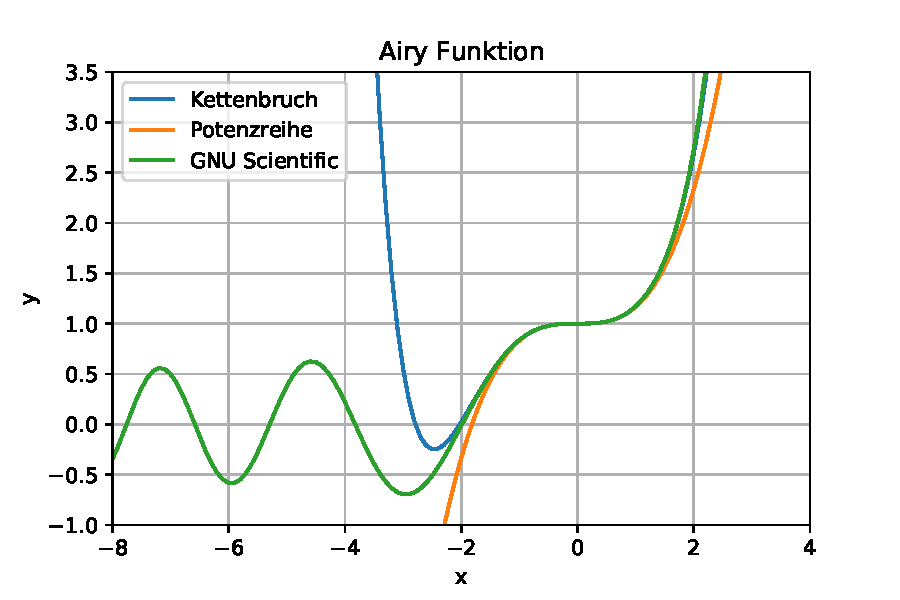
\includegraphics[width=0.8\textwidth]{papers/0f1/images/konvergenzAiry.pdf}
    \caption{Konvergenz nach drei Iterationen, dargestellt anhand der Airy Funktion zu den Anfangsbedingungen $\operatorname{Ai}(0)=1$ und $\operatorname{Ai}'(0)=0$.
    \label{0f1:ausblick:plot:airy:konvergenz}}
\end{figure}

\begin{figure}
    \centering
    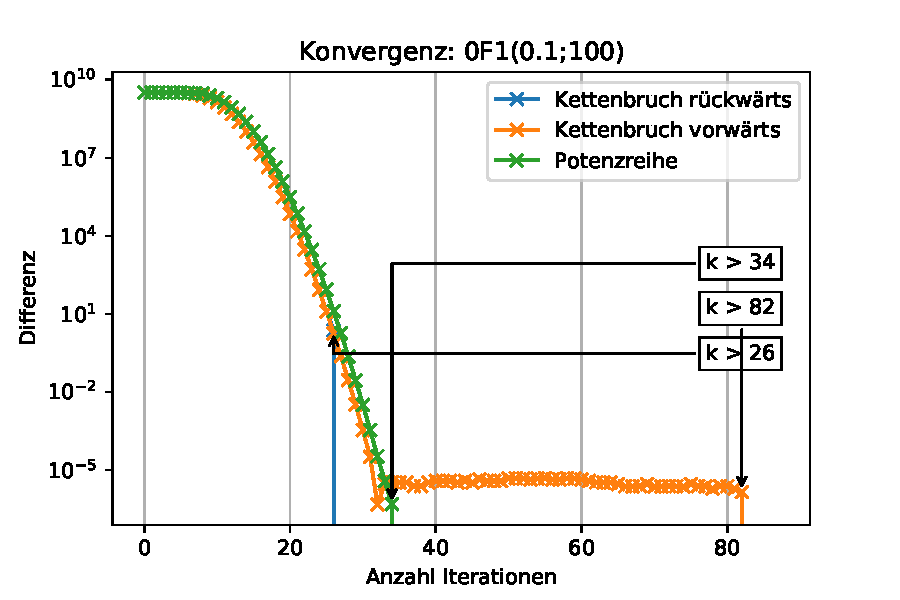
\includegraphics[width=0.8\textwidth]{papers/0f1/images/konvergenzPositiv.pdf}
    \caption{Konvergenz mit positivem $z$; Logarithmisch dargestellter absoluter Fehler.
    \label{0f1:ausblick:plot:konvergenz:positiv}}
\end{figure}

\begin{figure}
    \centering
    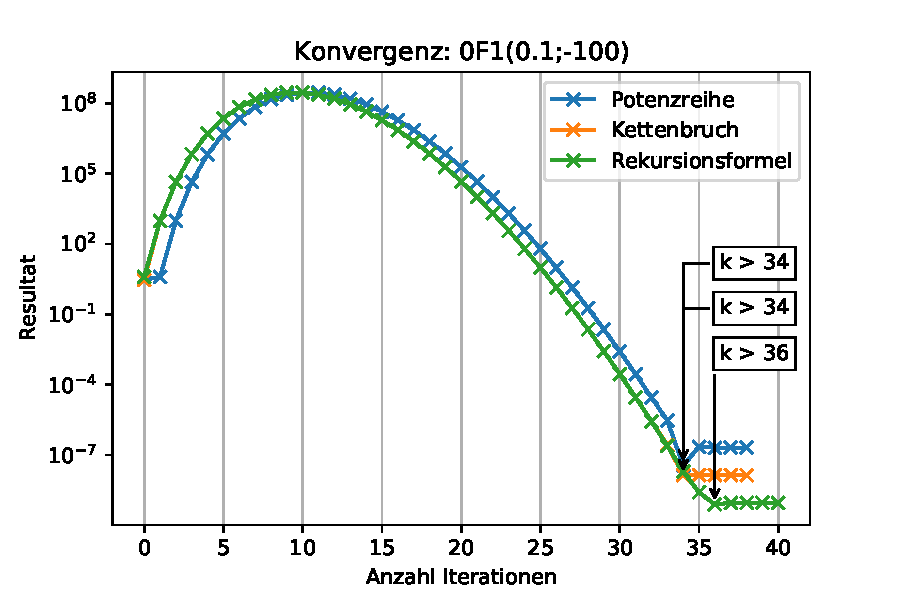
\includegraphics[width=0.8\textwidth]{papers/0f1/images/konvergenzNegativ.pdf}
    \caption{Konvergenz mit negativem $z$; Logarithmisch dargestellter absoluter Fehler.
    \label{0f1:ausblick:plot:konvergenz:negativ}}
\end{figure}

\begin{figure}
    \centering
    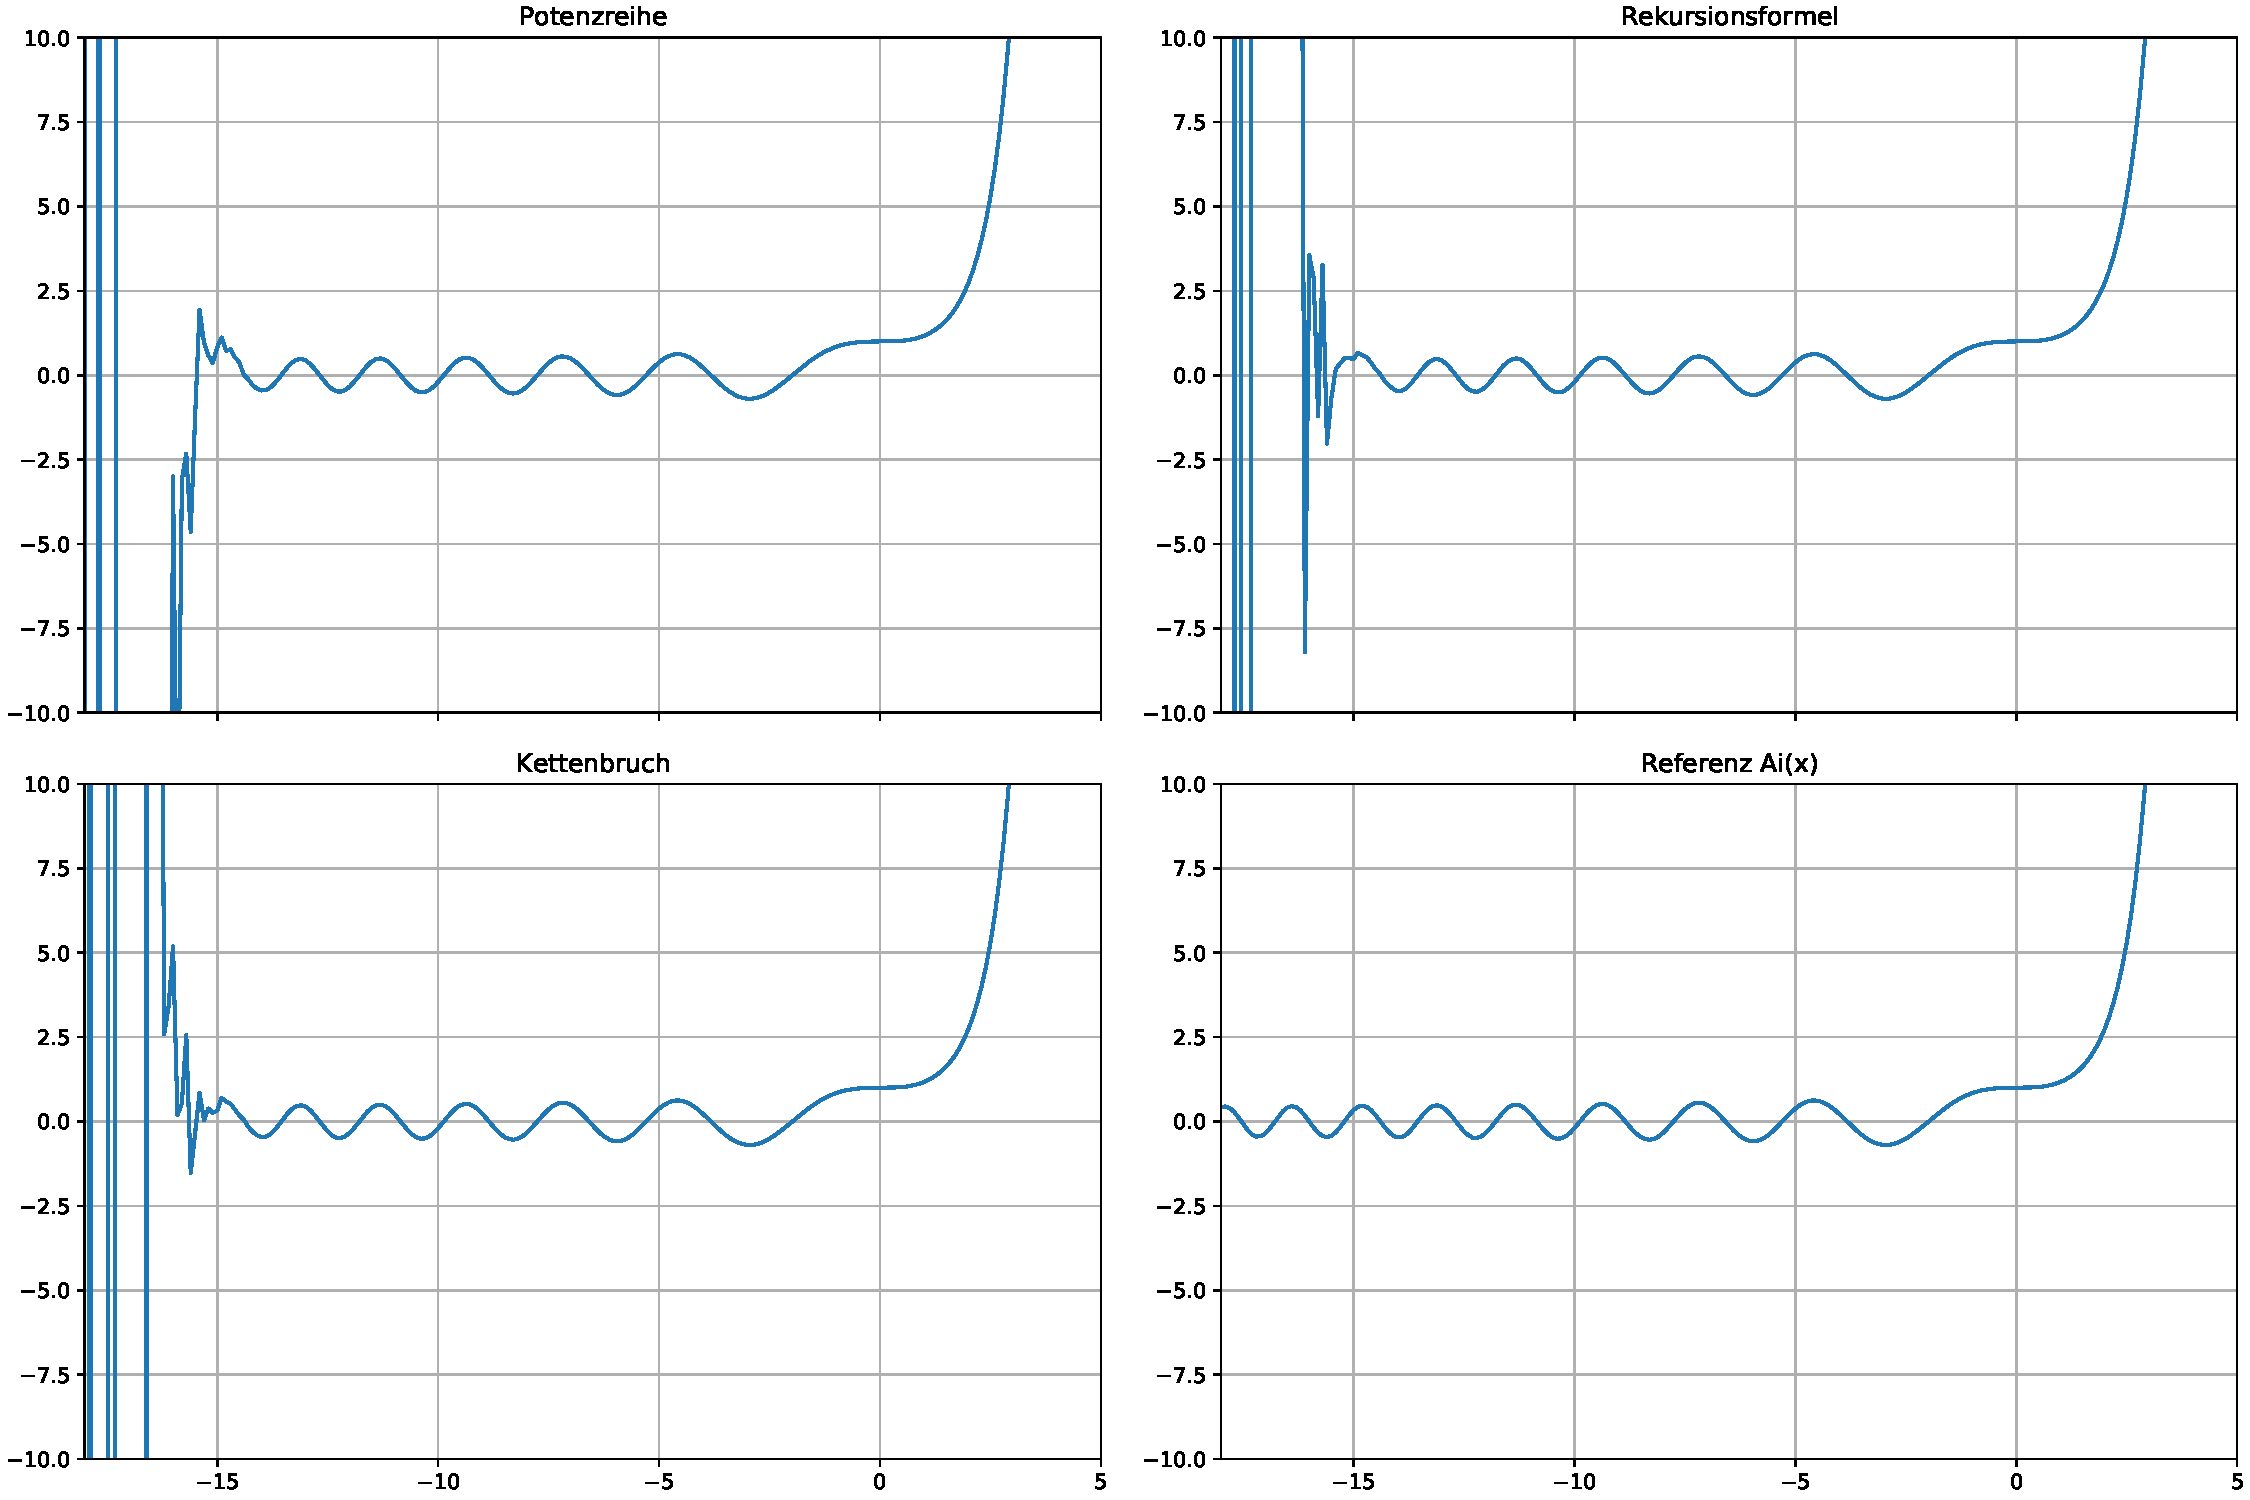
\includegraphics[width=1\textwidth]{papers/0f1/images/stabilitaet.pdf}
    \caption{Stabilität der drei Algorithmen verglichen mit der Referenz Funktion $\operatorname{Ai}(x)$.
    \label{0f1:ausblick:plot:airy:stabilitaet}}
\end{figure}

